\subsection{Session}

The \gls{cpe} needs to keep the user authenticated while navigating through the management interface, this is generally done with \gls{http} Cookies \cite{rfc6265}.

By analyzing the requests made by the browser when accessing the interface of \glspl{cpe} 4, 6, and 7, it was found that the cookies contain only 8 to 10 characters, as shown on Figure \ref{figure:cpe_cookies}. It seems to be risky, but given that the sessions are short lived and that the \gls{http} server is slow, hardly a brute-force attack would succeed.

\begin{figure}[h]
    \centering
    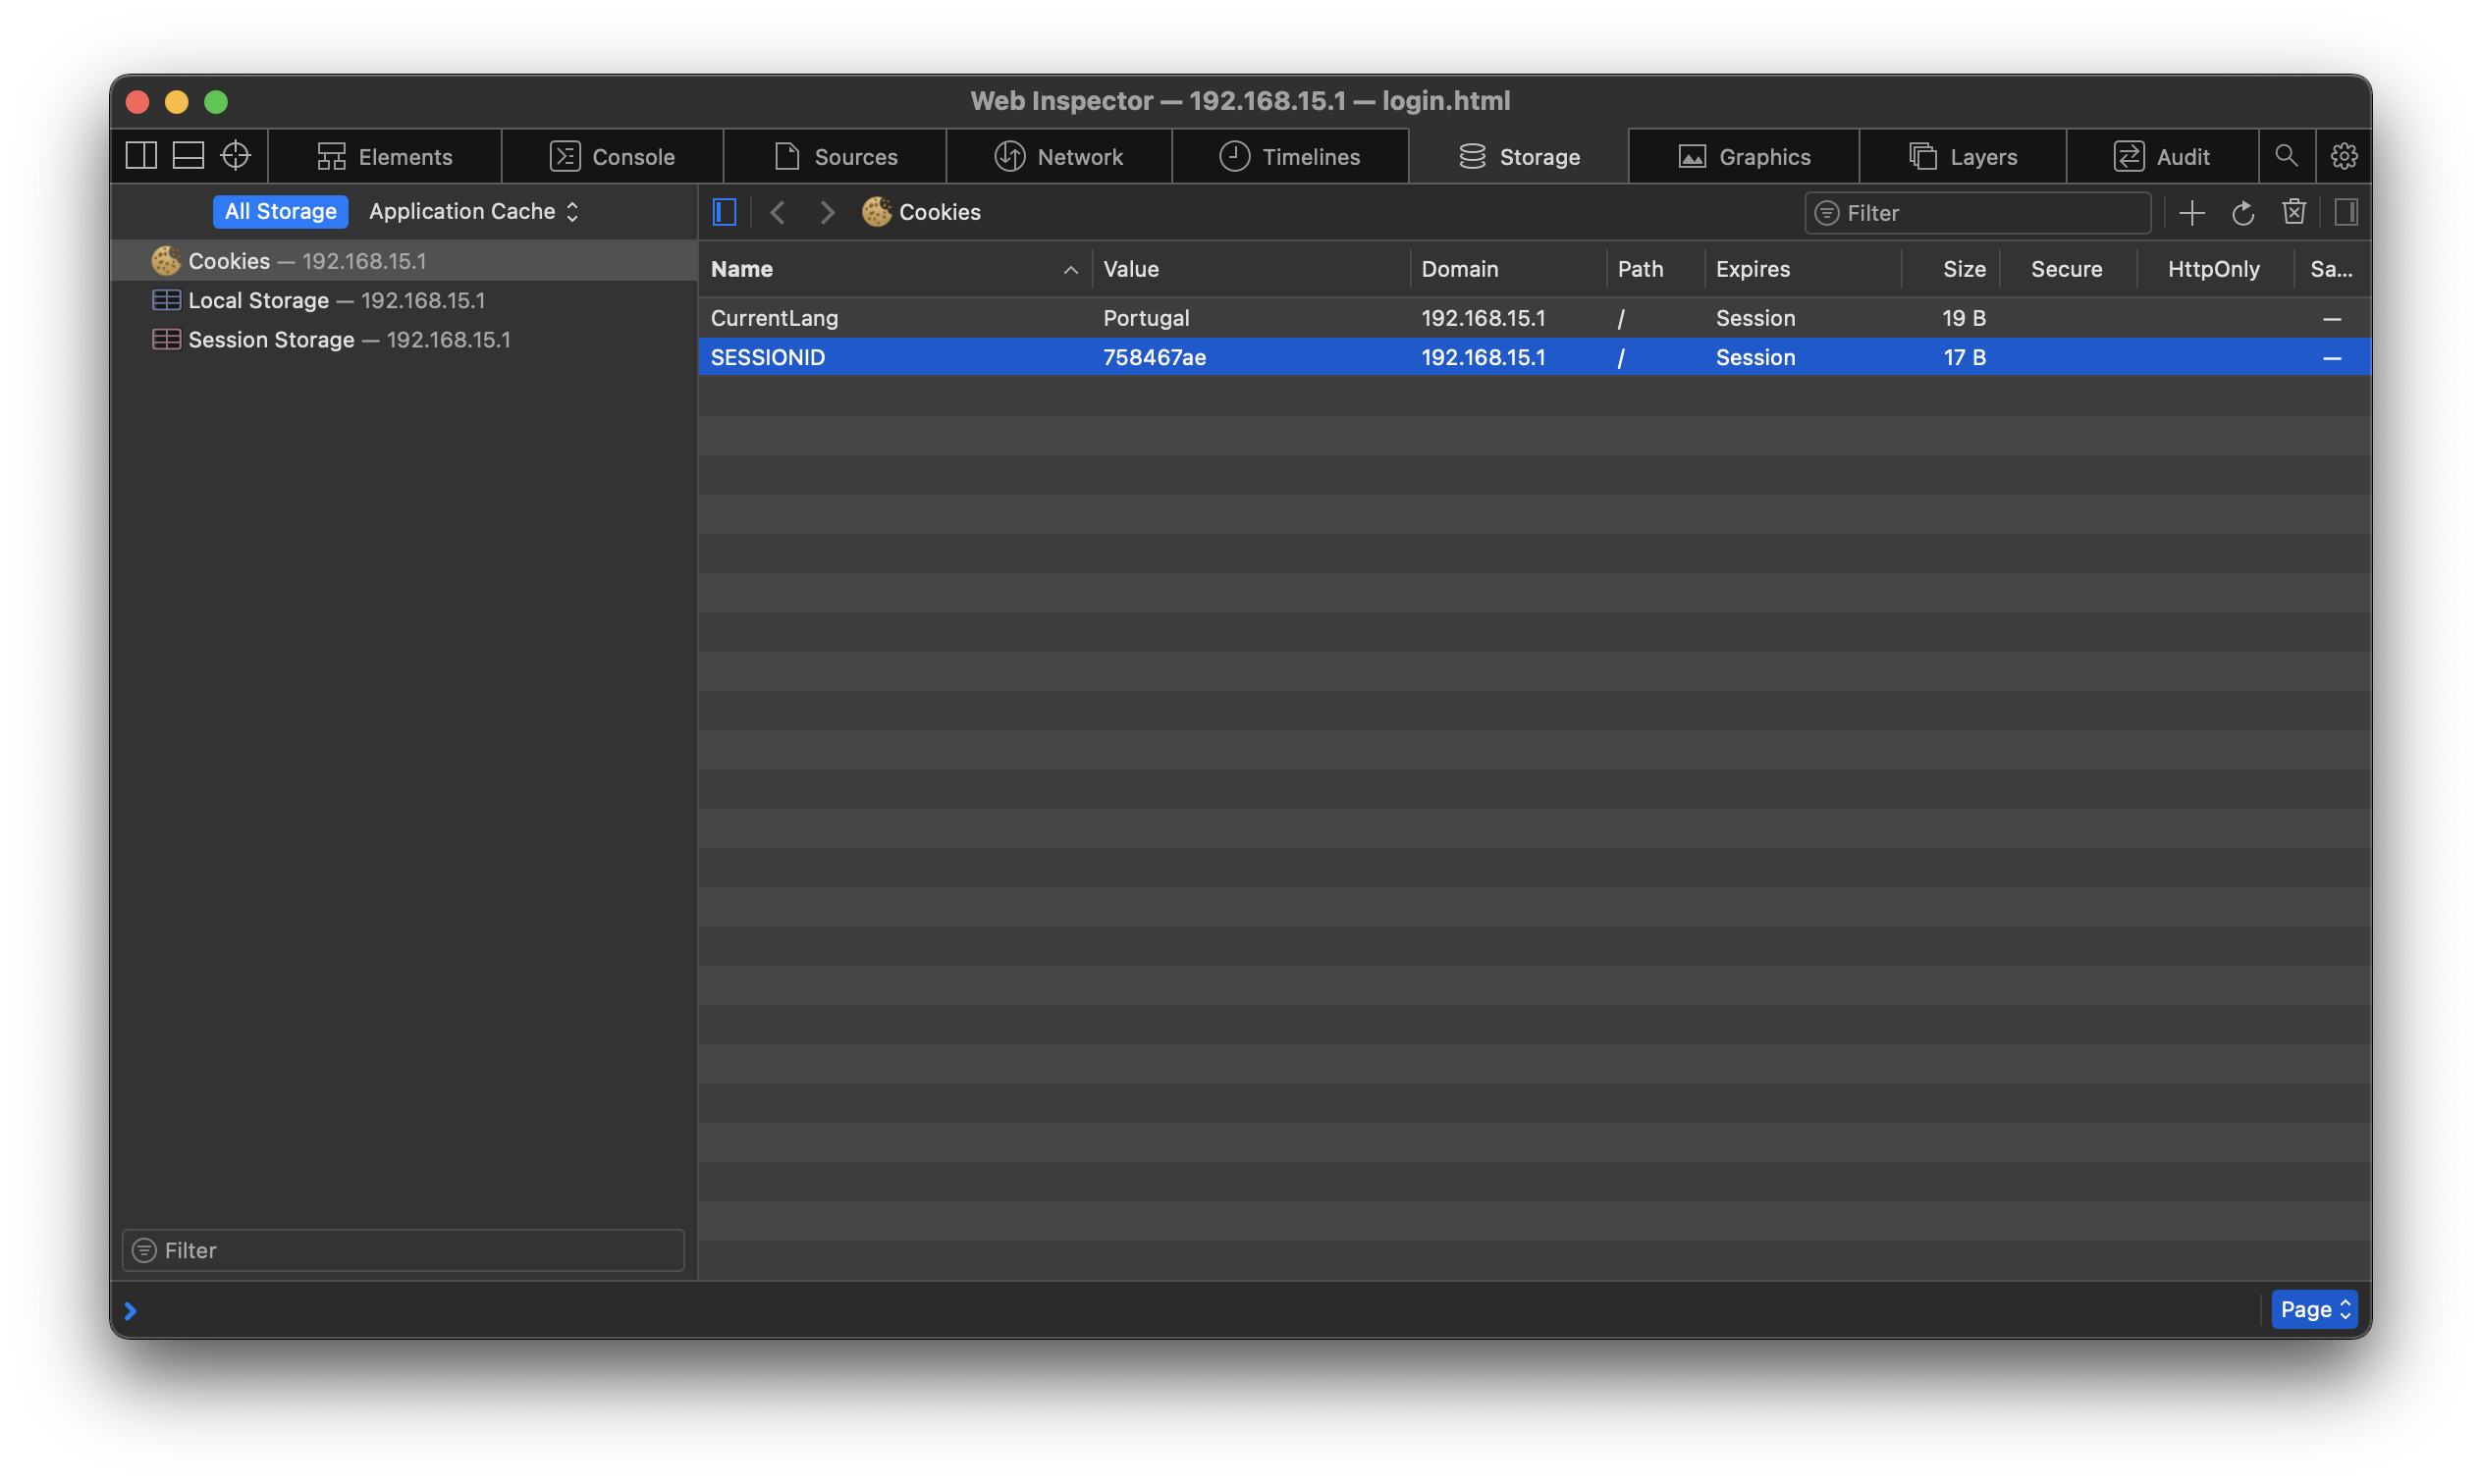
\includegraphics[width=\linewidth]{contents/http-management-interface-analysis/session/cpe-cookies.png}
    \caption{Cookies of the \gls{cwmp} \gls{http} Management Interface}
    \label{figure:cpe_cookies}
\end{figure}

Strangely, no cookie, authorization token, or any other method of keeping the user’s session was found on the captured requests of \glspl{cpe} 0 and 1. After performing some tests, it was identified that the \gls{cpe} authenticates the client based on its \gls{ip}. If another client on the network is able to hijack the \gls{ip} address of an authenticated user, it may gain access over the \gls{cpe}’s management interface.

\FloatBarrier
